\section{Desarrollo}

\subsection{Inducción matemática}

Inducción matemática es una técnica utilizada para probar declaraciones o proposiciones.
La idea es similar a la de hacer caer varias piezas de dominó.
\begin{figure}[htb]
    \centering
    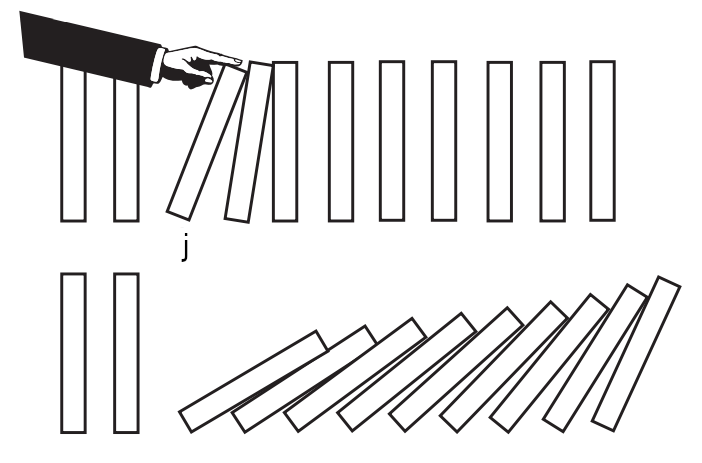
\includegraphics[width=7cm]{images/dominoes-fall}
    \caption{Fichas de dominó cayendo.}
    \label{fig:figure}
\end{figure}
Si cada pieza está lo suficientemente cerca de la anterior y hacemos caer la primera, entonces todas las piezas eventualmente van a caer.
Cuando queremos demostrar que una proposición se cumple sobre números naturales, la idea es la misma.
Dicho de otro modo, la inducción nos permite demostrar una propiedad en \textbf{infinitos números} con \textbf{pasos finitos}.

\begin{principle.box}{Inducción simple}{}
    Sea el entero $j$ y $S(n)$ una proposición sobre el entero $n$ con $n \geq j$,
    \begin{itemize}
        \item[i)] si $S(j)$ es cierto, y
        \item[ii)] para cada entero $k \geq j$, $S(k) \implies S(k + 1)$,
    \end{itemize}
    entonces $S(n)$ es cierta para todo $n \geq j$.
\end{principle.box}
Asi por ejemplo, si tenemos $j = 1$ y una proposición $T(n)$ cumple las dos condiciones anteriores,
entonces $T(n)$ se cumple para todo natural $n$, lo más común en la mayoría de los problemas es demostrar una propiedad
a partir de $j = 1$ o $j = 0$.

Es importante mencionar el vocabulario utilizado en la inducción matemática, el cual nos permite moldear una solución.
\begin{enumerate}
    \item \textbf{Paso base:} Identificar y validar el primer entero que cumple, $S(j)$ cierto.
    \item \textbf{Hipótesis de inducción:} Formular y tomar la proposición como cierta para un entero dado, $S(k)$ cierto.
    \item \textbf{Tesis de inducción:} Identificar la proposición a validar, $S(k + 1)$ cierto.
    \item \textbf{Paso inductivo:} Demostrar por medio de argumentos que la hipótesis implica a la tesis, $S(k) \implies S(k + 1)$.
\end{enumerate}
Hay varias maneras de interpretar la hipótesis y la tesis, por ejemplo
\begin{itemize}
    \item lo que sabemos y lo que buscamos,
    \item lo que tenemos y lo que debemos,
    \item entradas (input) y salidas (output),
\end{itemize}
entre otros, de cualquier modo todos siguen el objetivo de transformar la hipótesis en argumentos para demostrar la tesis.

Hay situaciones donde demostrar que una propiedad $S(n + 1)$ es verdadera no basta con solo tomar a $S(n)$ como cierto,
puesto que estas proposiciones a menudo dependen de la validez de más de un elemento anterior, dicho de otro modo,
necesitamos más información para demostrar la propiedad, para ello utilizamos la inducción fuerte.
\begin{principle.box}{Inducción fuerte}{}
    Sea $j$ un entero y $S(n)$ una proposición sobre el entero $n \geq j$.
    Si
    \[
        \forall k \geq j, \quad \left(\forall m < k,\ S(m)\right) \implies S(k),
    \]
    entonces $S(n)$ es cierta para todo $n \geq j$.
\end{principle.box}
La expresión $\left(\forall m < k,\ S(m)\right) \implies S(k)$ con $k \geq j$, es equivalente a la expresión
\[
    \left(S(j) \land S(j + 1) \land \cdots \land S(k - 1)\right) \implies S(k).
\]
Cuando $k = j$ de manera lógica obtenemos $S(j)$ cierto, lo cual es equivalente al paso base de la inducción simple,
por lo tanto, no es difícil notar que la inducción fuerte es el caso general de la inducción simple.

Veamos un ejemplo, que ilustra estos principios.
\begin{example}
    Hallar el $n_0 \in \nonnegativeSet{\Z}$ tal que cualquier entero $n \geq n_0$ cumple $n = 3i + 5j$ para algunos
    $i,j \in \nonnegativeSet{\Z}$.
\end{example}
\begin{solution}
    Haciendo unas algunas pruebas, encontramos que
    \begin{align*}
        &0 = 3\cdot 0 + 5\cdot 0 && 5 = 3\cdot 0 + 5\cdot 1 && 10 = 3\cdot 0 + 5\cdot 2\\
        &1\ \text{no cumple} && 6 = 3\cdot 2 + 5\cdot 0 && 11 = 3\cdot 2 + 5\cdot 1\\
        &2\ \text{no cumple} && 7\ \text{no cumple} && 12 = 3\cdot 4 + 5\cdot 0\\
        &3 = 3\cdot 1 + 5\cdot 0 && 8 = 3\cdot 1 + 5\cdot 1 && 13 = 3\cdot 1 + 5 \cdot 2\\
        &4\ \text{no cumple} && 9 = 3\cdot 3 + 5\cdot 0 && \text{etc ...}
    \end{align*}
    Es decir, a partir de $n_0 = 8$ notamos que los enteros siguientes empiezan a cumplir la propiedad \textbf{\small(paso base)}.
    Sea la proposición $S(n) : $ ``existen $i,j \in \nonnegativeSet{\Z}$ tales que $n = 3i + 5j$'' y supongamos que
    para un entero $k \geq 8$, $S(8), S(9), \ldots, S(k)$ son todos ciertos \textbf{\small(hipótesis de inducción)},
    entonces vamos a demostrar que $S(k + 1)$ también es cierto \textbf{\small(tesis de inducción)}.
    Se distinguen dos casos,
    \begin{itemize}
        \item $k = 8,9,10$, los cuales sabemos son ciertos y
        \item $k \geq 11$, de donde obtenemos que $8 \leq k - 3 \leq k$.
    \end{itemize}
    Por la hipótesis sabemos que existen $i_0,j_0 \in \nonnegativeSet{\Z}$ tales que $k - 3 = 3 i_0 + 5 j_0$, por lo tanto
    $k = 3 (i_0 + 1) + 5j_0$ donde $i = i_0 + 1$ y $j = j_0$ \textbf{\small(paso inductivo)}.
    Luego, $S(n)$ se cumple para todo entero $n \geq 8$.
\end{solution}


\subsection{Descenso infinito de Fermat}

Sigamos con otro principio, uno bastante intuitivo.
\begin{principle.box}{Buen orden}{}
    Para todo subconjunto no vacío de los naturales, este debe tener un elemento mínimo.
\end{principle.box}
De igual manera, es fácil pensar que un subconjunto no vacío de los números naturales debe tener un elemento máximo,
por consiguiente, cualquier subconjunto no vacío de los naturales debe tener un elemento mínimo y máximo.

Al trata de problemas en específicos, a menudo utilizamos estas nociones del principio de Buen orden, lo cual podemos
formalizar con el siguiente axioma.
\begin{axiom}[Axioma del Orden]
    Si $M$ es un conjunto de $n$ números reales distintos, entonces podemos escribirlo como $M = \{x_1,x_2,\ldots,x_n\}$
    con $x_1 < x_2 < \ldots < x_n$.
\end{axiom}
Las demostraciones por el principio del buen orden a menudo implica realizar una prueba por contradicción, en este texto
no abordaremos a detalle este principio, pero se invita a investigar más de este tema.
Esta noción de orden será de útilidad con el siguiente y último principio.

El descenso infinito proviene de resolver ecuaciones diofánticas indeterminadas, el matemático Pierre de Fermat
(1601-1665) utilizó este método hace unos 400 años cuando demostró que no existen soluciones enteras positivas
para\footnote{Se recomienda al lector buscar la solución de Fermat, para enrriquecer su lectura.} $x^4 + y^4 = z^4$.

\begin{principle.box}{Descenso infinito de Fermat}{}
    Sea $k \in \nonnegativeSet{\Z}$ y $S(n)$ una proposición sobre $n$,
    \begin{enumerate}
        \item[i)] si $S(k)$ no es cierto, y
        \item[ii)] para todo $m > k$, $S(m) \implies S(r)$ con $m > r > k$,
    \end{enumerate}
    entonces $S(n)$ no se cumple para ningún $n\geq k$.
\end{principle.box}
Podemos entender el descenso infinito de fermat metafóricamente con una escalera, si para alcanzar un escalón más alto es necesario
pasar primero uno más bajo, pero no existe un escalón más bajo en la escalera, entonces es imposible subir a ningún escalón.

Veamos dos variantes o casos concretos de este principio, útiles en el estudio de las ecuaciones diofánticas.
\begin{enumerate}
    \item[i)] No existe una secuencia $n_1 > n_2 > n_3 > \ldots$ estrictamente decreciente de enteros no negativos.
    \item[ii)] Si se tiene la secuencia $n_1\geq n_2 \geq n_3 \geq \ldots$ de enteros no negativos, entonces existe un $k \geq 1$ tal que $n_k = n_{k+1} = n_{k + 2} = \cdots$.
\end{enumerate}

Cabe destacar que los principios de Inducción matemática, Buen orden y Descenso infinito son de hecho equivalentes en
el conjunto de los enteros no negativos.
Con lo cual, si tomamos uno es posible demostrar con este los dos restantes\footnote{Se recomienda al lector investigar cómo son esas demostraciones}.

\begin{example}
    Probar que la ecuación $x^2 + y^2 = 3z^2$ no tiene soluciones $(x,y,z)$ en enteros positivos cuando $z \neq 0$.
\end{example}
\begin{solution}
    Supongamos que hay al menos una solución $(x_1,y_1,z_1)$ con $z_1 > 0$, es claro que en módulo 3 llegamos a $x_1^2+y_1^2 \modulo{0}{3}$.
    Como los cuadrados perfectos solo dejan resto $0$ o $1$ en módulo tres, necesariamente $x_1^2\equiv y_1^2 \modulo{0}{3}$,
    por lo cual $x_1 = 3x_2$, $y_1 = 3y_2$ con $x_1 > x_2$ y $y_1 > y_2$.

    Al reemplazar en la ecuación $9x_2^2+9y_2^2=3z_1^2 \iff 3(x_2^2+y_2^2)=z_1^2 \iff 3 \mid z_1^2 \iff 3 \mid z_1$.
    Si tomamos $z_1 = 3z_2$ con $z_1 > z_2$, entonces
    \[
        x_2^2+y_2^2=3z_2^2.
    \]
    Es decir, hemos encontrado una nueva solución $(x_2,y_2,z_2)$ a la ecuación original.
    Al analizar esta solución, obtendríamos otra nueva solución $(x_3,y_3,z_3)$, de la misma manera, aplicando este proceso
    obtendríamos soluciones $(x_4,y_4,z_4)$, $(x_5,y_5,z_5)$, $(x_6,y_6,z_6)$ y así sucesivamente.
    Sin embargo, esto implica que
    \begin{align*}
        x_1 > x_2 > x_3 > \cdots, \quad
        y_1 > y_2 > y_3 > \cdots \quad \text{y} \quad
        z_1 > z_2 > z_3 > \cdots.
    \end{align*}
    Lo cual es imposible, luego la ecuación original no tiene soluciones.
\end{solution}




\subsection{Ejercicios y problemas}

Ejercicios y problemas para el autoestudio.

\subsubsection{Inducción}
\begin{exercise}
    Hallar el $n_0 \in \nonnegativeSet{\Z}$ tal que $\forall n \geq n_0,\ n = 5i + 6j$ con $i,j \in \nonnegativeSet{\Z}$.
\end{exercise}

\begin{exercise}
    Probar para todo $n \in \N$ que el número $A_n = 3^n - 2n^2 - 1$ es múltiplo de $8$.
    Además, si $3\nmid n$, entonces $A_n$ es múltiplo de 24.
\end{exercise}

\begin{problem}
    Probar $\forall n \in \N$ que las ecuaciones tienen soluciones enteras
    \begin{align*}
        1)\ x^2 + y^2 = z^n, && 2)\ (x^2 + y^2)(u^2 + v^2 + w^2) = 2009^n.
    \end{align*}
\end{problem}

\begin{problem}
    Resolver $x_1^2 + x_2^2 + \dots + x_{2002}^2 = 1335\left(x_1 + x_2 + \dots + x_{2002}\right)$ en enteros positivos distintos
\end{problem}



\subsubsection{Descenso infinito}
\begin{exercise}
    Encuentre todas las soluciones enteras de la ecuación $a^2 - 2b^2 = 0$.
\end{exercise}

\begin{exercise}
    Hallar todos los números enteros $a,b,c$ tales que $a^2 = 2b^2 + 3c^2$.
\end{exercise}

\begin{exercise}
    Probar que $x^2 + y^2 = 3(m^2 + n^2)$ no tiene soluciones enteras positivas.
\end{exercise}

\begin{exercise}
    Hallar las soluciones $(a,b) \in \nonnegativeSet{\Z}$ para $a^2 + b^2 + c^2 = a^2 b^2$.
\end{exercise}

\begin{exercise}
    Resolver en enteros de la ecuación $2005x^3 = y^3 + 25z^3$.
\end{exercise}

\begin{exercise}
    Muestre que no hay enteros positivos $x,y,z$ tal que $x^2 + 10y^2 = z^2$.
\end{exercise}

\begin{problem}
    ¿Hay soluciones racionales para $x^2+ y^2 + z^2 + 3(x+y+z) + 5 = 0$?
\end{problem}

\begin{problem}
    Hallar las triplas $(x,y,z) \in \N$ que cumplen $x^3 + 3y^3 + 9z^3 - 3xyz = 0$.
\end{problem}

\begin{problem}
    Hallar todos los enteros $x,y,z$ para los cuales $x^2 + y^2 + z^2 - 2xyz = 0$.
\end{problem}

\begin{problem}
    Resolver en enteros positivos la ecuación $m^2 - mn - n^2 = \pm 1.$
\end{problem}



\subsubsection{Buen orden}
\begin{exercise}
    Hallar el mínimo, máximo y orden, de los siguientes conjuntos.
    \begin{multicols}{2}
        \begin{enumerate}
            \item $A = \{4,7,6,3,78,10,5, 1,6\}$.
            \item Los divisores de 121.
            \item Múltiplos de 3 entre 20 y 80.
            \item Los primos impares menores a 50.
            \item Los primos entre 50 y 100.
            \item Cubos perfectos menores de 200
        \end{enumerate}
    \end{multicols}
\end{exercise}